
\section{How much needs to change, and how fast?}

The Paris Climate Accord commits its signatories to limiting global warming to ``well below'' 2.0$^\circ$C and preferably to within 1.5$^\circ$C \cite{UnitedNations2015}. 2.0$^\circ$C has long been considered an essential goal to avoid severe damage to earth systems and possible run-away effects\cite{Meinshausen2009, Allen2009, IPCC2014}. The inclusion of the more audacious 1.5$^\circ$ C ambition was an unexpected but welcome and important development in the 2015 negotiations leading up to the Paris Climate Accord. A 2018 report from the Intergovernmental Panel of Climate Change (IPCC), called the SR15 in their jargon, emphasized what's at stake in the difference between these two targets\cite{IPCC2018_SPM}. 
\begin{figure}[h!]
	\centering
	\includegraphics[width=0.8\textwidth]{01_Intro/fig/reasons_for_concern.png}
	\caption{Severity of climate change risks increases from present warming (1$^\circ$C) to 1.5$^\circ$C and further to 2.0$^\circ$C of warming. From the IPCC SR15 (2018) summary for policy makers, ref. \cite{IPCC2018_SPM}}
	\label{fig:RFC}
\end{figure}
Some of the differences in the risks posed by 2.0 vs 1.5$^\circ$C are shown in Figure \ref{fig:RFC}, taken from that report. Risks posed to ecosystems and human quality of life are much higher at 2.0$^\circ$C than 1.5$^\circ$C.

\textit{Carbon budgets} are a powerful, if also a bit simplistic\cite{Peters2018}, way to think about the societal changes necessary to stay within a global warming target. The carbon budget remaining to have a 67\% chance of confining global warming to 1.5$^\circ$C is about 160 GtC (570 Gt \ch{CO2})\cite{IPCC2018_ch2}. In other words, with 160 additional gigatons of carbon added to the air as \ch{CO2}, 67\% of climate simulations predict that the average temperature will remain within 1.5$^\circ$C of the pre-industrial baseline. (Temperature increase is approximately linear with cumulative \ch{CO2} emissions to a point\cite{IPCC2018_ch2}, so the carbon budget to limit global warming to 2$^\circ$C is about 300 GtC.)

The 1.5$^\circ$C carbon budget is more than 1/3 of the cumulative emissions up to today, but only approximately 15 years at present global emissions rate, which is just over 10 GtC/yr\cite{LeQuere2018}. This means that emissions will have to fall very rapidly to keep climate change within safe levels. The question of how rapidly emissions need to fall depends, more than anything else, on whether and to what extent we will, in the future, be willing to pay the bill of removing \ch{CO2} from the atmosphere that we emit today. Figure \ref{fig:paths}, from the same IPCC report, summarizes this point. 
\begin{figure}[h!]
	\centering
	\includegraphics[width=0.85\textwidth]{01_Intro/fig/pathways_to_1p5C.png}
	\caption{\ch{CO2} emissions pathways consistent with max 1.5$^\circ$C global warming involve emissions reductions of $\approx 50$\% by 2030 and to net zero by around 2050. IPCC SR15 (2018) Chapter 2, ref. \cite{IPCC2018_ch2}}
	\label{fig:paths}
\end{figure}

Here, a large number of simulations (referred to as pathways) involving changing anthropogenic emissions are fed to a climate model which predicts among other things the evolution of the global mean surface temperature between now and the year 2100. The figure illustrates pathways for which global warming in the year 2100 is less than or equal to 1.5$^\circ$C. It is important to note that in all of the pathways that involve significant \ch{CO2} removal from the atmosphere, the temperature overshoots then comes down again to 1.5$^\circ$C of warming by the end of the century. All pathways that avoid such an overshoot of 1.5$^\circ$C involve steep reductions in emissions starting more or less immediately. They tend to involve an approximately 50\% reduction in \ch{CO2} emissions from 2010 levels by 2030, and net zero emissions by 2050\cite{IPCC2018_ch2}. This can be used as a working, easy-to-remember policy guideline:
\begin{definition}
A policy is consistent with the Paris Agreement if it leads to a 50\% reduction (relative to 2010) in \ch{CO2} emissions by 2030, and net zero emissions by 2050. \label{d:Paris}
\end{definition}

It is important to note that, while climate change is a global problem, policies are set more locally. Of course, if every country makes its policies in line with Definition \ref{d:Paris}, then it will be fulfilled globally. However, in reality, some countries will fall behind, and it should be considered the responsibility of developed countries with the capacity to do so to meet and exceed the criterion in Definition \ref{d:Paris}. Developed countries have this responsibility because both their emissions per capita and their cumulative contribution to today's climate change are disproportionately high\cite{Ritchie2019a}. More importantly, all capable countries should enact policies in line with Definition \ref{d:Paris} in order to minimize their contribution to any eventual overshoot of 1.5$^\circ$C warming, to set an example, and to develop expertise that can then accelerate the required changes in slower countries.

In this context, the European Union's present target of ``At least 40\% cut in greenhouse gas emissions compared with 1990''\cite{EC_2030}, which is only a 30\% cut compared to 2010\cite{Ritchie2019a}, falls short, but will hopefully be tightened soon. Proudly, Denmark's new government has put in place a target of 70\% reduction by 2030 with respect to 1990 (60\% reduction with respect to 2010)\cite{CHN_70p}. Denmark's target is in line with the Paris Agreement by Definition \ref{d:Paris}. 
%\vspace{1cm}

%I have had the privilege of interacting with climate activists who often prioritize a concept of \textit{climate justice}, with whom I agree often but not always. While the fact that fossil fuel companies have spent decades gambling our collective future by intentionally funding the spread of disinformation\cite{HeadsInSand} inspires rage and should be litigated when possible; and while figuring out how to fairly allocate the world's remaining carbon budget is important\cite{Wegge2019}; and while individuals in a democracy undeniably carry a responsibility for their collective fate; I think it is essential that none of these distract us from the most urgent priority, which is finding and implementing the answers to this simple question (based on Definition \ref{d:Paris}): % move to Foreword.

%Definition \ref{d:Paris} means that a top priority moving forward is finding and implementing answers to this simple question:

The question, then, that should be on all of our minds, is:

\begin{question}
How can we cut emissions to half or less by 2030? \label{q:how}
\end{question}

This is not an especially easy question to answer, since the combustion of fossil fuels has become a stubbornly fundamental cornerstone of the Western material lifestyle, which for better or worse is well on its way to spreading to the rest of the world. Almost everything we do, whether it's turning on a light, eating a burger, buying a new shirt, heating our home in the winter, commuting to work, charging a computer, or visiting an exciting new place is coupled to the release of greenhouse gases. Of course not all these activities do equal damage, as will be illustrated more thoroughly in Chapter \ref{ch:Impact}, but modern economies are so complexly interconnected that it is not reasonable to expect individuals to make these judgments. Furthermore, however high the degree of individual freedom in our societies, many of the important consumption decisions in our lives are made for us by institutions or cultural norms. This is not to discount the importance of awareness and engagement, and the responsibility individuals in a democracy carry for their collective fate. But the answers to Question \ref{q:how} are best found and implemented on levels starting from cities and up through regions, nations, and international organizations.

\begin{figure}[h!]
	\centering
	\includegraphics[width=0.6\textwidth]{01_Intro/fig/sectors.png}
	\caption{Global 2010 greenhouse gas emissions by sector, from the IPCC's AR5, 2014, ref. \cite{IPCC2014}}
	\label{fig:sectors}
\end{figure}

Figure \ref{fig:sectors}, from the IPCC's previous report (AR5, from 2014)\cite{IPCC2014} divides global green-house gas emissions in 2010 up into sectors. The largest single source of greenhouse-gas emissions is due to electricity generation (25\%), followed by the grouping of agriculture, forestry, and other land use (AFOLU, 24\%), and then industry (21\%). 

The fact that electricity generation is the largest single source of greenhouse-gas emissions is in fact incredibly good news, since there are a number of technologies that can generate electricity with little to no greenhouse-gas emissions. Wind turbines and photovoltaics (solar panels) are becoming the most important \ch{CO2}-free electricity sources due to unlimited scalability (in contrast to hydro and geothermal power), broad societal acceptance (in contrast to nuclear fission), and technological maturity (in contrast to a number of emerging technologies)\cite{BNEF2018, Creutzig2017}. 
\begin{figure}[h!]
	\centering
	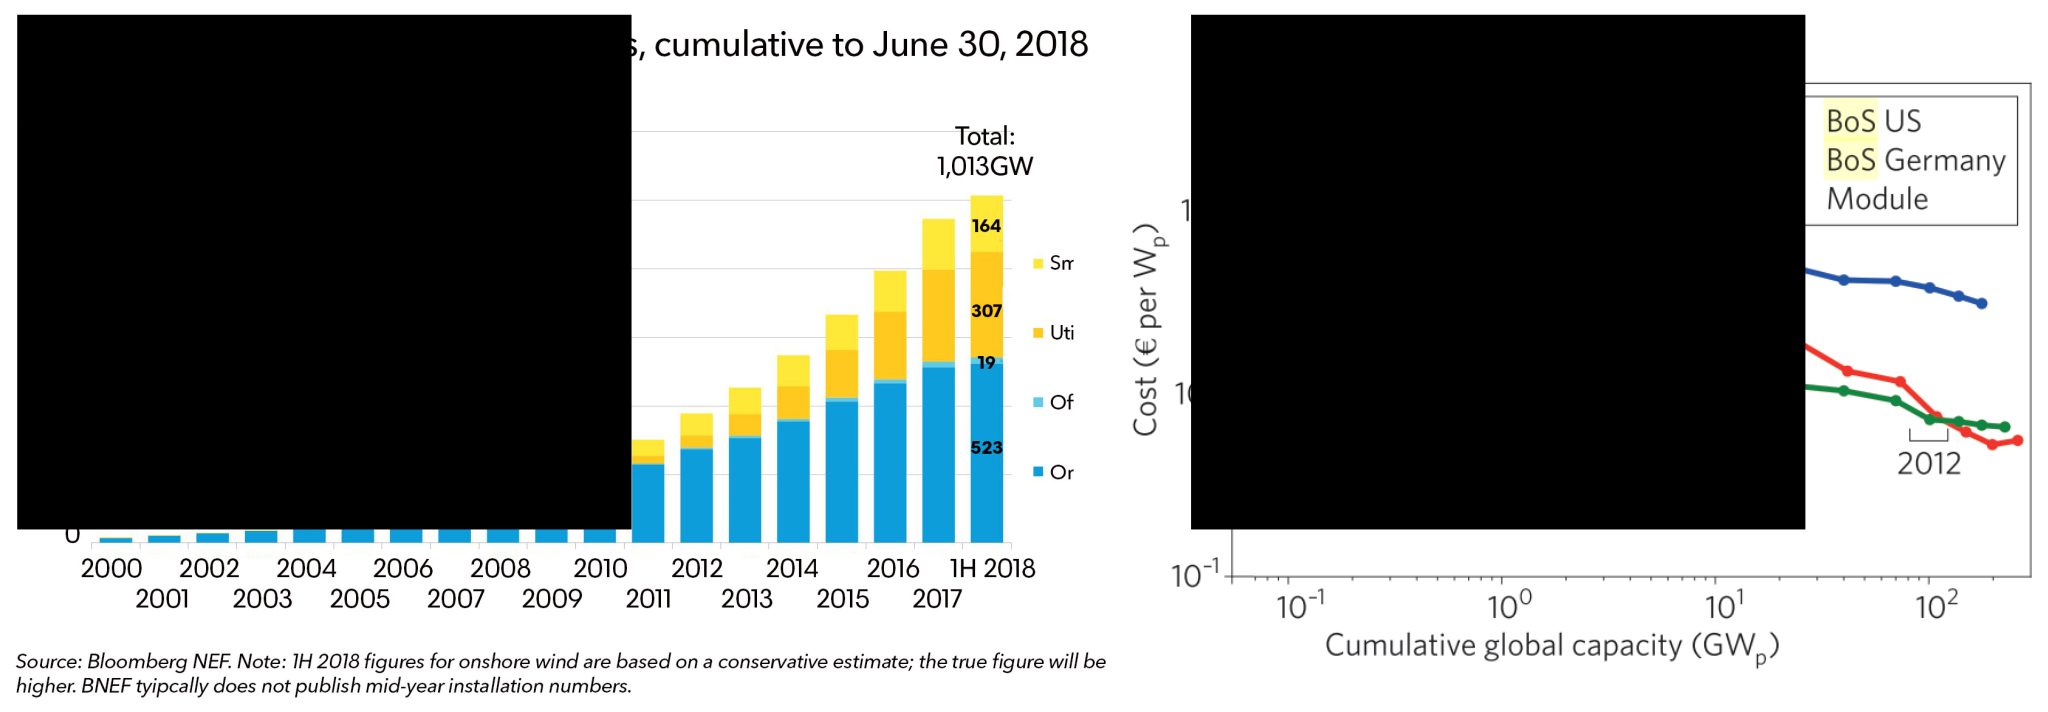
\includegraphics[width=\textwidth]{01_Intro/fig/renewables.png}
	\caption{Rapid progress of renewables. \textbf{(a)}, Growing installed capacity of wind and solar, from Bloomberg New Energy Finance (BNEF), 2019, ref. \citen{BNEF2018}. \textbf{(b)}, Solar learning curve including module and balance of system (BOS) prices, adapted from Creutzig et al, 2017, ref. \citen{Creutzig2017}.}
	\label{fig:renewables}
\end{figure}
Figure \ref{fig:renewables} illustrates the rapid growth in wind and solar energy. The combined installed capacity of wind and solar passed 1 TW\cite{BNEF2018} in 2018, corresponding to approximately one sixth of total electricity generation capacity \cite{IRENA2019}. The actual share of global electricity generated by wind and solar in 2018, though, is only 7.5\% (2000 out of 27000 TWh)\cite{Enerdata2019}, slightly less than half as large a portion as installed capacity. This discrepancy is no quirk in the data - it is a fundamental drawback of wind turbines and solar panels: they only generate electricity when the wind is blowing or the sun is shining, respectively. More on that in a moment. Nonetheless, wind and solar are expected to keep growing as a share of renewable energy generation for some time. The levelized cost per energy is already less than fossil fuels in most places and continues to fall as the total installed capacity increases\cite{Bloomberg2016, Creutzig2017}. Wind and solar electricity generation is an incredible ongoing success story. Not least because reducing the carbon intensity of electricity works without requiring anything of the consumer, and thus represents a strategy to mitigate the risks of climate change with minimal disruption of society. Indeed, the most promising way to decarbonize many the other sectors in Figure \ref{fig:sectors} is to \textit{electrify} them. 

Wind and sunlight may come for free, and building wind and solar capacity may be cheaper than fossil fuel generation, but in the end the changes required by Definition \ref{d:Paris} still don't come for free. And this is because of the \textit{intermittency problem}, namely the fact that the wind and the sun are not kind enough to blow and shine exactly when we might need the electricity. It turns out that there are no cheap solutions to this problem, which will be described in more detail in the next Section. 

One possible rough answer to Question \ref{q:how} is then:

\begin{enumerate}
	\item Install wind and solar as much and as fast as possible to decarbonize electricity production!
	
	\item Electrify everything that can possibly electrified! The main opportunities are in Transport (14\% of direct \ch{CO2} emissions), Buildings (6.4\%), and Industry (21\%). \label{it:electrify}

	\item Solve the problem of intermittancy. \label{it:intermittant}
	
	\item Do less of the things that are hard to electrify, and \textbf{stop doing the greenhouse-gas-emitting things that can't be electrified!} \label{it:sacrifice}
%	\begin{itemize}
%		\item Stop eating meat
%		\item Stop flying
%	\end{itemize}
\end{enumerate}

These four steps can and must be advanced simultaneously.
\footnote{Note that bio-energy is not included in this suggested answer at all. This is in part because bio-energy is out of the scope of this Thesis, but mainly because the climate impact of substituting fossil fuels with biofuels is highly scrutinized. Use of land for bio-energy, especially forest bio-energy may actually \textit{increase} \ch{CO2} concentrations in the atmosphere to 2050 and beyond compared to burning fossil fuels and leaving the biomass to grow.\cite{Searchinger2018, Bentsen2017}. As such, it is a terrible mistake that the EU counts forest biomass as carbon-free renewable energy!}
The challenges are both technological and social. The technological challenges, today, are primarily in Items \ref{it:electrify} and \ref{it:intermittant}. The solutions for solving the intermittancy problem and for electrifying other sectors, are overwhelmingly based on \textit{electrochemistry}, the subject of the next Section and the motivation for this PhD Project.

The societal challenges lie in getting people to accept the costs of implementing these technologies, either through taxes or through increased prices in electricity and other products; and in making lifestyle changes where electricity can't help, or can't help fast enough (Item \ref{it:sacrifice}). Notable carbon-intensive activities that cannot be electrified in the foreseeable future, if at all, include meat consumption (8.5\% of global emissions \cite{Caro2017}) and air travel (2\% of global emissions and growing\cite{CarbonBrief_aviation}, and probably a much larger portion of the emissions for which the reader of this Thesis is responsible). A powerful and in-discriminant way to promote all of the steps above within the framework of a free-market economy and to get individuals to make the necessary sacrifices is a universally applied \ch{CO2} tax. This is the favored method by economists\cite{CarbonTax_Economist}, but has to be high enough to influence both corporate and individual behavior.

The need for everyone to accept sacrifices is where the climate crisis poses a challenge for capitalistic liberal democracies. On the one hand, such societies feature political and economic systems which all too easily fall to the temptation of serving short-term interests. On the other hand, the free inquiry of science and the engagement of the public at the core of their values is what has succeeded in bringing climate change to the top of the agenda in Europe. There is no guarantee we will be able to make the necessary changes fast enough to keep climate change from delivering the fatal wound to Fukuyama's dream. But there is reason to be optimistic.



%There is almost certainly no getting around it: For the first three steps to be sufficient, it would require 100\% renewable electricity generation together with more than 60\% overall of all the transport, industry, and buildings direct emissions being eliminated by electrification by 2030. Complete decarbonization of electricity by 2030 is probably possible but expensive: the larger the renewable energy penetration, the more expensive it is to solve the intermittency problem\cite{Budschak2013, Sgobbi2016}. But a 60\% decarbonization of the other sectors, especially industry, seems difficult. 
 






